% !Mode::"TeX:UTF-8"

% -------------------- Information --------------------

\newcommand{\TITLE}{非线性方程求根}
\newcommand{\AUTHOR}{Jason}
\newcommand{\SUBJECT}{数值分析理论课}
\newcommand{\KEYWORDS}{}

% -------------------- Packages --------------------

\documentclass[a4paper, 12pt]{ctexart}
\usepackage{amsmath}
\usepackage{amssymb}
% \usepackage{amsthm} % 定理格式 由ntheorem代替.
\usepackage{authblk} % 作者 (见校赛论文).
\usepackage{array}
\usepackage{bigfoot} % to allow verbatim in footnote.
\usepackage{bm} % \bm for bold symbols.
\usepackage{boldline} % 长表格表格线加粗.
\usepackage{caption} % 题注.
\usepackage{commath} % abs, norm
\usepackage{enumerate}
% \usepackage{enumitem} 用enumerate包代替.
\usepackage{fancyhdr} % 脚注.
\usepackage{filecontents}
\usepackage{flafter} % 不让float出现在定义之前的地方.
\usepackage{float} % 你们这帮float给我乖乖听话 HHHHHHHHHHH.
\usepackage[T1]{fontenc} % Bera Mono Font
\usepackage{fontspec} % 字体.
\usepackage{graphicx}
\usepackage{hyperref}
\usepackage{lastpage}
\usepackage{letltxmacro} % \let
\usepackage{lipsum}
\usepackage{listings} % 排版程序语言.
\usepackage{longtable} % 长表格.
\usepackage{makecell} % 表格线加粗 \Xhline{1.2pt}.
\usepackage{mathtools} % \xleftrightarrow.
\usepackage{mathrsfs} % \mathscr
\usepackage{multirow} % 合并单元格.
\usepackage[square, numbers, sort&compress]{natbib} % 引用.
\usepackage[thmmarks, amsmath, thref]{ntheorem} % 定理格式.
\usepackage[section]{placeins} % 使图像不会显示在别的部分 若过于严格则换成[below].
\usepackage{stackrel} % 上下写 见校赛论文.
\usepackage{subcaption} % subcaption and subfigure
% \usepackage{SUBSubsubsection}
\usepackage{titlesec} % Section标题格式.
\usepackage{varioref} % For Cross References.
\usepackage[dvipsnames]{xcolor} % 颜色声明.
\usepackage{xfrac} %\sfrac{}{}
\usepackage[all, cmtip]{xy} % Commutive diagram.

% Require `ntheorem'

\usepackage[mathlines, edtable]{lineno} % Line numbers.
    %\begin{edtable}{tabular}[<args>] <entries> \end{edtable}

% Require `xcolor'

\usepackage[numbered, framed]{matlab-prettifier}
\usepackage{pgfplots}
\usepackage{pgfplotstable}
\usepackage{tikz}

% Incompatible with `matlab-prettifier'

\usepackage[printwatermark]{xwatermark} % Foreground Watermarks.

% -------------------- Settings --------------------

% Title

\title{\TITLE}
\author{\AUTHOR}
\date{\today}

% Package: caption

\captionsetup{
    margin    =   6pt,
    font      =   small,
    labelfont =   bf
}

% Package: ctex

\setCJKfamilyfont{fzstk}{FZShuTi} % 方正舒体
\newcommand{\fzstk}{\CJKfamily{fzstk}}

% Package: fancyhdr

\setlength{\headheight}{15pt}
\lhead{Copyright \copyright\ \AUTHOR}
\rhead{Page \thepage\ of \pageref{LastPage}}

% Package: graphicx

\graphicspath{{resources/}} % 图像文件目录

% Package: hyperref

\hypersetup{
    linktoc             =   all,
    colorlinks          =   true,
    linkcolor           =   cyan,
    anchorcolor         =   black,
    citecolor           =   green,
    filecolor           =   cyan,
    menucolor           =   red,
    runcolor            =   filecolor,
    urlcolor            =   magenta,
	pdftitle           	=   {\TITLE},
	pdfauthor          	=   {\AUTHOR},
	pdfsubject         	=   {\SUBJECT},
	pdfcreator			=	{Visual Studio Code},
	pdfproducer			=	{XeLaTeX with documentclass ctexart},
	pdfkeywords        	=   {\KEYWORDS},
    bookmarksnumbered   =   true,
    pdfstartview        =   FitH,
    pdfpagelayout       =   OneColumn
}

% Package: lineno

\renewcommand{\linenumberfont}{\normalfont\scriptsize\sffamily}

\let\oldlstinputlisting\lstinputlisting
\renewcommand{\lstinputlisting}[2][\empty]{
    \par\nolinenumbers\oldlstinputlisting[#1]{#2}\linenumbers\par
}

\let\oldlstlisting\lstlisting
\let\oldendlstlisting\endlstlisting
\renewenvironment{lstlisting}
    {\par\nolinenumbers\oldlstlisting}
    {\oldendlstlisting\endnolinenumbers\par}

\let\oldtable\table
\let\oldendtable\endtable
\renewenvironment{table}
    {\par\nolinenumbers\oldtable}
    {\oldendtable\endnolinenumbers\par}

% Package: listings

%% Title

\renewcommand\lstlistingname{代码}
\renewcommand\lstlistlistingname{代码}

%% Lstinline with color box

\LetLtxMacro{\oldlstinline}{\lstinline}
\renewcommand{\lstinline}[2][]{\colorbox{lightgray}{\oldlstinline[#1]{#2}}}
\newcommand{\matlabinline}[1]{
    \lstinline[style=MATLAB-editor, basicstyle=\mlttfamily]{#1}}

\lstset{
    breaklines=true,
    backgroundcolor=\color{lightgray},
    basicstyle=\scriptsize,
    inputpath=resources/,
    numbers=left,
    numberstyle={\color{black!33}\scriptsize\sffamily},
    xleftmargin=2em,
    xrightmargin=2em
}

% Package: ntheorem

%% Theorem
\newtheorem{theorem}{Theorem}[section]
\newtheorem{lemma}[theorem]{Lemma}
\newtheorem{corollary}[theorem]{Corollary}
%% Problem
\theoremstyle{plain}
\newtheorem{problem}{Problem}[section]
%% Proposition
\newtheorem{proposition}{Proposition}[section]
%% Conjecture
\newtheorem{conjecture}[proposition]{Conjecture}
%% Definition
\theoremstyle{plain}
\theoremheaderfont{\bfseries}
\theorembodyfont{\rmfamily}
\newtheorem{definition}{Definition}[section]
%% Note
\theoremstyle{plain}
\theoremheaderfont{\itshape}
\theorembodyfont{\itshape}
\newtheorem{note}{Note}[section]
%% Proof
\theoremstyle{nonumberplain}
\theoremheaderfont{\itshape}
\theorembodyfont{\upshape}
\theoremseparator{.}
\theoremsymbol{\ensuremath{\square}}
\newtheorem{proof}{Proof}
%% Solution
\theoremsymbol{\ensuremath{\blacksquare}}
\newtheorem{solution}{Solution}

% Package: pgfplot

\pgfplotsset{width=7cm, compat=1.16}

% Package: pgfplotstable

\pgfplotstableset{
    every head row/.style={before row=\Xhline{1.2pt},after row=\hline},
    every last row/.style={after row=\Xhline{1.2pt}}
}

% Package: varioref

\renewcommand{\reftextbefore}
    {on the \reftextvario{preceding page}{page before}}
\renewcommand{\reftextafter}
    {on the \reftextvario{following}{next} page}
\renewcommand{\reftextfacebefore}
    {on the \reftextvario{facing}{preceding} page}
\renewcommand{\reftextfaceafter}
    {on the \reftextvario{facing}{next} page}
\renewcommand{\reftextfaraway}[1]
    {on page \pageref{#1}}

%% Label formats

\labelformat{lstlisting}{代码#1}
\labelformat{equation}{式(#1)}
\labelformat{figure}{图#1}
\labelformat{table}{表#1}

% Package: xwatermark

\newsavebox\mybox
\savebox\mybox{\tikz[color=cyan, opacity=0.2]\node{\fzstk\SUBJECT};}
\newwatermark*[
    allpages,
    angle=45,
    scale=6,
    xpos=-20,
    ypos=15
]{\usebox\mybox}

% -------------------- General new commands --------------------

\DeclareMathAlphabet{\mathsfsl}{OT1}{cmss}{m}{sl}

\DeclareMathOperator{\arcosh}{arcosh}
\DeclareMathOperator{\Arcosh}{Arcosh}
\DeclareMathOperator*{\Beta}{B}
\DeclareMathOperator{\Log}{Log}
\DeclareMathOperator*{\real}{Re}
\DeclareMathOperator*{\image}{Im}

% Expectation

\newcommand{\expect}{\operatorname{E}\expectarg}
\DeclarePairedDelimiterX{\expectarg}[1]{(}{)}{
    \ifnum\currentgrouptype=16 \else\begingroup\fi
    \activatebar#1
    \ifnum\currentgrouptype=16 \else\endgroup\fi
}

\newcommand{\innermid}{\nonscript\;\delimsize\vert\nonscript\;}
\newcommand{\activatebar}{
    \begingroup\lccode`\~=`\|
    \lowercase{\endgroup\let~}\innermid
    \mathcode`|=\string"8000
}

\newcommand*{\BC}{\mathbb{C}}
\newcommand*{\BR}{\mathbb{R}}
\newcommand*{\diff}{\mathop{}\!\mathrm{d}}
\newcommand*{\matr}[1]{\ensuremath{\mathsfsl{#1}}} % italic sans serif
\newcommand*{\me}{\mathrm{e}}
\newcommand*{\mi}{\mathrm{i}}
\newcommand*{\restrict}[1]{\raisebox{-.5ex}{$\vert$}_{#1}}
\newcommand*{\vect}[1]{\bm{#1}}

% -------------------- Specific new commands --------------------



% -------------------- Document --------------------

\begin{document}

    % -------------------- Title Page --------------------

    \maketitle
    \thispagestyle{empty}
    \pagenumbering{roman}

    % -------------------- Abstract Page --------------------

    % -------------------- Contents --------------------

    % \newpage
    % \tableofcontents

    % -------------------- Body --------------------

    \newpage
    \pagestyle{fancy}
    \pagenumbering{arabic}
    \linenumbers

    \begin{problem}
        用牛顿法或弦截法计算方程$f(x)=3x^{3}-8x^{2}-8x-11=0$的某个近似根,
        使误差具有精度$10^{-4}$.
    \end{problem}

    \begin{solution}
        我们取迭代初值$x_{0} = 0$, 实现MATLAB代码如下:

        \lstinputlisting[
            caption=na7\_10.m,
            style=MATLAB-editor,
            basicstyle=\mlttfamily\scriptsize
        ]{na7_10.m}

        其中牛顿法代码如下:

        \lstinputlisting[
            caption=newton\_iteration.m,
            style=MATLAB-editor,
            basicstyle=\mlttfamily\scriptsize
        ]{newton_iteration.m}

        最终解得\matlabinline{x=3.6667}, \matlabinline{iter=36}.
    \end{solution}
    
    \begin{problem}
        用牛顿法, 割线法等求解下面各个问题, 列表比较各算法的性能.
        \begin{equation}
            \begin{aligned}
                &\text{\upshape (a)} x^{5}-3x-10=0,
                &&\text{\upshape (b)} \sin{10x}+2\cos{x}-x-3=0,\\
                &\text{\upshape (c)} x+\arctan{x}=3,
                &&\text{\upshape (d)} (x+2)\log{(x^{2}+x+1)}+1=0.
            \end{aligned}
        \end{equation}
    \end{problem}

    \begin{solution}
        取初值$x_{0}=0$, $x_{1}=1$, 并令$K=1000$, $\varepsilon=10^{-6}$.
        实现MATLAB代码如下:

        \lstinputlisting[
            caption=na7\_13.m,
            style=MATLAB-editor,
            basicstyle=\mlttfamily\scriptsize
        ]{na7_13.m}

        其中割线法代码如下:

        \lstinputlisting[
            caption=secant\_method.m,
            style=MATLAB-editor,
            basicstyle=\mlttfamily\scriptsize
        ]{secant_method.m}

        单点割线法代码如下:

        \lstinputlisting[
            caption=single\_point\_secant\_method.m,
            style=MATLAB-editor,
            basicstyle=\mlttfamily\scriptsize
        ]{single_point_secant_method.m}

        各算法在我们选定的初值和允许误差下, 收敛所需的迭代次数如下表:

        \begin{table}[H]
            \begin{center}
                \caption{迭代次数表}
                \pgfplotstabletypeset[
                    columns/算法/.style={string type},
                ]{
                    算法 a b c d
                    牛顿迭代法 268 15 4 13
                    割线法 23 5 4 18
                    单点割线法 1000 1000 10 1000
                }
            \end{center}
        \end{table}

        可见单点割线法效果不是很好.
    \end{solution}

    \begin{problem}
        尝试用各种方法计算下面方程在区间$[-10, 10]$中的所有根:
        \begin{equation}
            \sum_{k=1}^{10}{k\me^{-\cos{kx}}\sin{kx}}=2.
        \end{equation}
    \end{problem}

    \begin{solution}
        先画图:
        \begin{figure}[H]
            \centering
            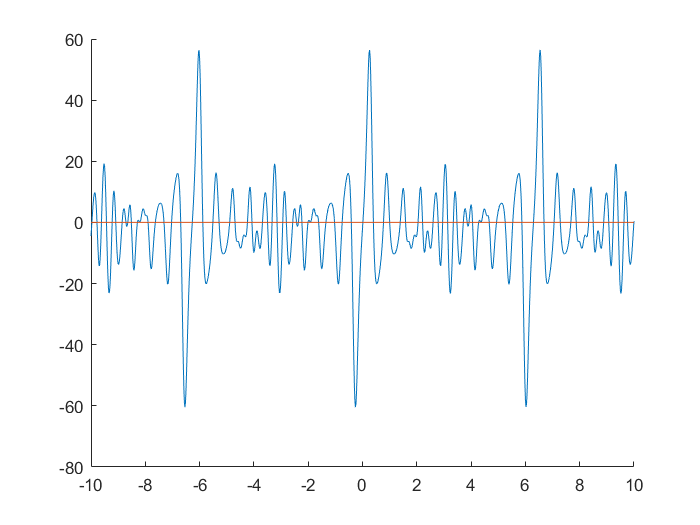
\includegraphics[scale=0.5]{naexp7_2.png}
            \caption{函数图像}
        \end{figure}

        MATLAB代码如下:

        \lstinputlisting[
            caption=naexp7\_2.m,
            style=MATLAB-editor,
            basicstyle=\mlttfamily\scriptsize
        ]{naexp7_2.m}
    \end{solution}
    
    % -------------------- Bibliography --------------------

    % \newpage
    % \bibliography{Principles_of_Mathematical_Analysis}
    % \bibliographystyle{plain}

\end{document}
